\documentclass[12pt]{article}
\usepackage{amssymb, amsmath, amsfonts, bm, graphicx, geometry}
\usepackage{tabularx, booktabs, float, enumitem, multicol, mathtools}
\usepackage{parskip} % Auto-manages paragraph spacing and removes indentations
\usepackage{siunitx}  % Eases typesetting of numbers and units

% US customary units
\DeclareSIUnit{\inch}{in}
\DeclareSIUnit{\foot}{ft}
\DeclareSIUnit{\yard}{yd}
\DeclareSIUnit{\mile}{mi}

\DeclareSIUnit{\slug}{slug}
\DeclareSIUnit{\lbm}{lbm}
\DeclareSIUnit{\lbf}{lbf}

\DeclareSIUnit{\psi}{psi}
\DeclareSIUnit{\psf}{psf}

\DeclareSIUnit{\gallon}{gal}
\DeclareSIUnit{\quart}{qt}
\DeclareSIUnit{\fahrenheit}{F}
\DeclareSIUnit{\rankine}{R}
\sisetup{
    per-mode = fraction
}
\usepackage{soul}
\usepackage{mathrsfs}

\geometry{margin=1in}

% Uppercase Volume with thicker, higher line
\newcommand{\vol}{\mathord{\text{\ooalign{\hidewidth $V$\hidewidth\cr\kern-0.5pt\raisebox{0.8ex}{\rule[0pt]{1em}{0.5pt}}}}}}

% Lowercase Volume with built-in shifts
\newcommand{\svol}{%
  \mathord{\text{\ooalign{%
    \hfil$v$\hfil\cr
    \hfil\rule[0.6ex]{0.8em}{0.5pt}\hfil
  }}}%
}

\begin{document}

\begin{center}
{\LARGE ESC-340 Fluid Mechanics \& Flow Systems HW\par}
\end{center}
\hrule
\vspace{1.5em}
\section*{\fbox{3.2 F = ma along a streamline}}
\textbf{Problem 3.2.1}\\
Air at $15^\circ\mathrm{C}$ flows steadily along a streamline from point (1) to point (2) with negligible viscous effects. The following conditions are measured: at point (1) $z_1=2\ \mathrm{m}$ and $p_1=0\ \mathrm{kPa}$; at point (2) $z_2=13\ \mathrm{m}$, $p_2=15\ \mathrm{N/m^2}$, $V_2=0$, and $\rho=1.225\ \mathrm{kg/m^3}$. Determine the velocity at point (1).

\textbf{Solution}
\begin{itemize}
    \item Since the flow is steady, incompressible, and inviscid, the Bernoulli equation can be applied.
    \[p_1+\frac{1}{2}\rho V_1^2+\gamma z_1=p_2+\frac{1}{2}\rho V_2^2+\gamma z_2\]
    \item Since $p_1=0$, $V_2=0$, and $\gamma=\rho g$,
    \[\frac{1}{2}\rho V_1^2+\rho gz_1=p_2+\rho gz_2\]
    or
    \[V_1^2=2\frac{p_2}{\rho}+2g(z_2-z_1)\]
    \[=\frac{2\left(15\ \frac{\mathrm{N}}{\mathrm{m}^2}\right)}{1.225\ \frac{\mathrm{kg}}{\mathrm{m}^3}}+2\left(9.81\ \frac{\mathrm{m}}{\mathrm{s}^2}\right)\left[(13\ \mathrm{m})-(2\ \mathrm{m})\right]\]
    \[=240.3\ \frac{\mathrm{m}^2}{\mathrm{s}^2}\]
    \item Thus,
    \[\sqrt{V_1^2}=\sqrt{240.3\ \frac{\mathrm{m}^2}{\mathrm{s}^2}}\]
    \[\boxed{V_1=15.5\ \frac{\mathrm{m}}{\mathrm{s}}}\]
\end{itemize}


\textbf{Problem 3.2.2}\\
SAE 30 oil $\left(\rho=912\ \frac{\mathrm{kg}}{\mathrm{m}^3}\right)$ flows steadily through a horizontal pipe. Determine the pressure gradient along the streamline required to accelerate the SAE 30 oil at a rate of $31\ \frac{\mathrm{m}}{\mathrm{s}^2}$.

\textbf{Solution}
\begin{itemize}
    \item The equation of motion for steady inviscid flow along the streamline direction is:
    \[-\gamma\sin\theta-\frac{\partial p}{\partial s}=\rho V\frac{\partial V}{\partial s}=\rho a_s\]
    \item Rearranging to solve for $\frac{\partial p}{\partial s}$ gives
    \[\frac{\partial p}{\partial s}=-\gamma\sin\theta-\rho a_s\]
    where $\theta=0$ since the pipe is horizontal.
    \item Thus,
    \[\frac{\partial p}{\partial s}=-\rho a_s\]
    \[=-\left(912\ \frac{\mathrm{kg}}{\mathrm{m}^3}\right)\left(31\ \frac{\mathrm{m}}{\mathrm{s}^2}\right)\]
    \[=-28000\left(\frac{\mathrm{N}}{\mathrm{m}^2}\right)\frac{1}{\mathrm{m}}\]
    or
    \[\boxed{\frac{\partial p}{\partial s}=-28\ \frac{\mathrm{kPa}}{\mathrm{m}}}\]
\end{itemize}

\section*{\fbox{3.3 F = ma normal to a streamline}}
\textbf{Problem 3.3.1}\\
Air ($\rho=0.00238\ \mathrm{slugs/ft^3}$) flows along a horizontal, curved streamline with a 23 ft radius with a speed of 108 ft/s. Determine the pressure gradient normal to the streamline.

\begin{center}
    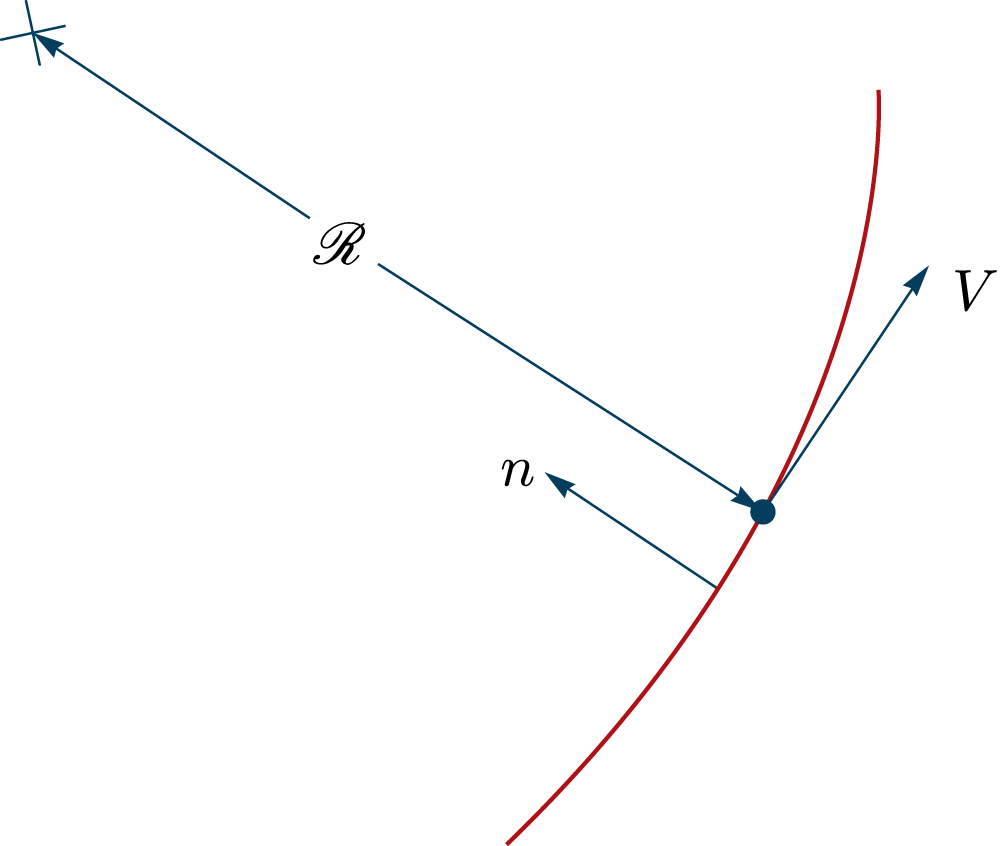
\includegraphics[width=0.3\textwidth]{3-3-1.png}
\end{center}

\textbf{Solution}
\begin{itemize}
    \item The equation of motion for steady inviscid flow normal to the streamline direction is:
    \[-\gamma\frac{dz}{dn}-\frac{\partial p}{\partial n}=\frac{\rho V^2}{\mathscr{R}}\]
    \item Rearranging to solve for $\frac{\partial p}{\partial n}$ gives
    \[\frac{\partial p}{\partial n}=-\gamma\frac{dz}{dn}-\frac{\rho V^2}{\mathscr{R}}\]
    where $\frac{dz}{dn}=0$ since the streamline is horizontal.
    \item Thus,
    \[\frac{\partial p}{\partial n}=-\frac{\rho V^2}{\mathscr{R}}\]
    \[=-\frac{\left(0.00238\ \frac{\mathrm{slugs}}{\mathrm{ft}^3}\right)\left(108\ \frac{\mathrm{ft}}{\mathrm{s}}\right)^2}{23\ \mathrm{ft}}\]
    \[=-1.21\ \frac{\mathrm{slug}}{\mathrm{ft}^2\cdot\mathrm{s}^2}\left[\frac{1\ \mathrm{lb}}{1\ \frac{\mathrm{slug}\cdot\mathrm{ft}}{\mathrm{s}^2}}\right]\]
    \[\boxed{\frac{\partial p}{\partial n}=-1.21\ \frac{\mathrm{lb}}{\mathrm{ft}^3}}\]
\end{itemize}


\textbf{Problem 3.3.2}\\
Water flows around the vertical two-dimensional bend with circular streamlines and constant velocity as shown in the figure below. If the pressure is 67 kPa at point (1), determine the pressure at point (2). Assume that the velocity profile is uniform as indicated.

\begin{center}
    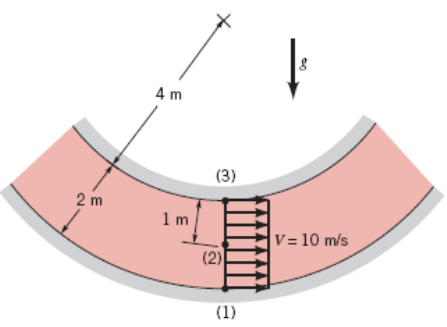
\includegraphics[width=0.4\textwidth]{3-3-2.png}
\end{center}

\textbf{Solution}
\begin{itemize}
    \item
    \[-\gamma\frac{dz}{dn}-\frac{\partial p}{\partial n}=\frac{\rho V^2}{R}\]
    with
    \[\frac{dz}{dn}=1\]
    and
    \[V=10\ \frac{\mathrm{m}}{\mathrm{s}}\]
    \item Thus, with $R=6-n$,
    \[\frac{dp}{dn}=-\gamma-\frac{\rho V^2}{6-n}\]
    or
    \[\int_{n=0}^{n=2}\frac{dp}{dn}\,dn=-\int_{n=0}^{n=2}\gamma\,dn-\int_{n=0}^{n=2}\frac{\rho V^2\,dn}{6-n}\]
    \item Since $\gamma$ and $V$ are constants
    \[p-p_1=-\gamma n-\rho V^2\int_{n=0}^{n}\frac{dn}{6-n}\]
    \item Thus,
    \[p=p_1-\gamma n-\rho V^2\ln\left(\frac{6}{6-n}\right)\]
    \item With $p_1=67\ \mathrm{kPa}$ and $n_2=1\ \mathrm{m}$:
    \[p_2=67\times10^3\ \mathrm{Pa}-9.8\times10^3\ \frac{\mathrm{N}}{\mathrm{m}^3}(1\ \mathrm{m})-999\ \frac{\mathrm{kg}}{\mathrm{m}^3}\left(10\ \frac{\mathrm{m}}{\mathrm{s}}\right)^2\ln\left(\frac{6}{5}\right)\]
    or
    \[\boxed{p_2=39\ \mathrm{kPa}}\]
\end{itemize}

\section*{\fbox{3.4 Physical interpretations and alternate forms of the Bernoulli equation}}
\textbf{Problem 3.4.1}\\
\textbf{(a)} Consider the inviscid, incompressible, steady flow of water shown below. From section A to B, the streamlines are straight. With $z_1=8\ \mathrm{m}$ and $z_2=15\ \mathrm{m}$, determine the pressure at (2) and the pressure at (1).

\begin{center}
    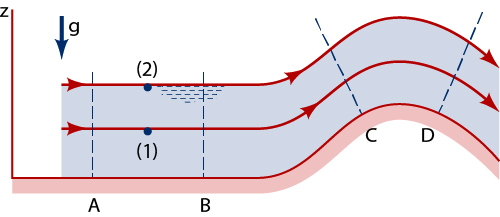
\includegraphics[width=0.5\textwidth]{3-4-1-a.jpeg}
\end{center}

\textbf{Solution}
\begin{itemize}
    \item Since (2) is on the surface and has the same pressure as the atmospheric pressure:
    \[\boxed{p_2=0\ \mathrm{kPa}}\]
    \item The Bernoulli equation applied across the streamlines is
    \[p+\rho\int\frac{V^2}{\mathscr{R}}\,dn+\gamma z=\text{constant across a streamline}\]
    where $\mathscr{R}=\infty$ for the portion between A and B since the streamlines are straight. Since the flow is inviscid, incompressible, and steady, the equation simplifies to:
    \[p+\gamma z=\text{constant}\]
    so
    \[p_1+\gamma z_1=p_2+\gamma z_2\]
    \item Since $p_2=0\ \mathrm{kPa}$, the equation becomes:
    \[p_1=\gamma(z_2-z_1)\]
    \item Thus,
    \[p_1=\left(1000\ \frac{\mathrm{kg}}{\mathrm{m}^3}\right)\left(9.8\ \frac{\mathrm{m}}{\mathrm{s}^2}\right)(15\ \mathrm{m}-8\ \mathrm{m})\left(\frac{1\ \mathrm{kPa}}{1000\ \mathrm{Pa}}\right)\]
    \[\boxed{p_1=68.60\ \mathrm{kPa}}\]
\end{itemize}

\textbf{(b)} From section C to D, the streamlines are curved. Describe the pressure variation between points (3) and (4). Is the pressure at point 3 less than, equal to, or greater than the hydrostatic pressure at point 3, $\gamma h_{4-3}$?

\begin{center}
    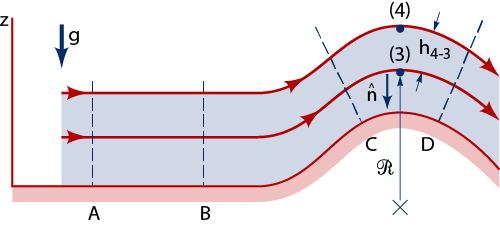
\includegraphics[width=0.5\textwidth]{3-4-1-b.jpeg}
\end{center}

\textbf{Solution}
\begin{itemize}
    \item The Bernoulli equation applied across the streamlines is
    \[p+\rho\int\frac{V^2}{\mathscr{R}}\,dn+\gamma z=\text{constant across a streamline}\]
    \item Since the flow is inviscid, incompressible, and steady, the equation simplifies to:
    \[p+\rho\int\frac{V^2}{\mathscr{R}}\,dn+\gamma z=\text{constant}\]
    \item Since $n=-z$
    \[p+\rho\int\frac{V^2}{\mathscr{R}}(-dz)+\gamma z=\text{constant}\]
    \item Applying the above between points (3) and (4) gives:
    \[p_3+\rho\int_C^{z_3}\frac{V^2}{\mathscr{R}}(-dz)+\gamma z_3=p_4+\rho\int_C^{z_4}\frac{V^2}{\mathscr{R}}(-dz)+\gamma z_4\]
    \item Since $p_4=0$ the equation becomes:
    \[p_3=\gamma(z_4-z_3)-\rho\int_{z_3}^{z_4}\frac{V^2}{\mathscr{R}}\,dz\]
    \item To evaluate the integral, we must know the variation of $V$ and $\mathscr{R}$ with $z$. Even without this detailed information, we note that the integral has a positive value. Thus, the pressure at (3) is less than the hydrostatic value, $\gamma h_{4-3}$, by an amount equal to $\rho\int_{z_3}^{z_4}\left(\frac{V^2}{\mathscr{R}}\right)\,dz$. This lower pressure, caused by the curved streamline, is necessary to accelerate the fluid around the curved path.
    \[\boxed{p_3<\gamma h_{4-3}}\]
\end{itemize}

\section*{\fbox{3.5 Static, stagnation, dynamic, and total pressure}}
\textbf{Problem 3.5.1}\\
Nitrogen ($0.00226\ \mathrm{slugs/ft^3}$) flows along a horizontal streamline. At a given point on the streamline, the static pressure is $-1.6\ \mathrm{psi}$ (i.e., a vacuum) and the velocity is $148\ \mathrm{ft/s}$. Determine the pressure at a stagnation point on the streamline.

\textbf{Solution}
\begin{itemize}
    \item An example streamline that satisfies the given conditions is shown below. Point 2 is a stagnation point since $V_2=0$.

    \begin{center}
        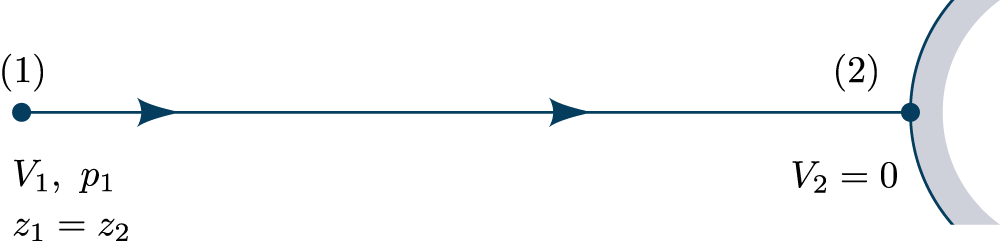
\includegraphics[width=0.5\textwidth]{3-5-1.png}
    \end{center}

    \item The Bernoulli equation is used to determine the pressure at the stagnation point.
    \[p_1+\frac{1}{2}\rho V_1^2+\gamma z_1=p_2+\frac{1}{2}\rho V_2^2+\gamma z_2\]
    where $z_1=z_2$ and $V_2=0$.
    \item Thus,
    \[p_2=p_1+\frac{1}{2}\rho V_1^2\]
    \[=\left(-1.6\ \frac{\mathrm{lb}}{\mathrm{in.}^2}\right)\left(144\ \frac{\mathrm{in.}^2}{\mathrm{ft}^2}\right)+\frac{1}{2}\left(0.00226\ \frac{\mathrm{slugs}}{\mathrm{ft}^3}\right)\left(148\ \frac{\mathrm{ft}}{\mathrm{s}}\right)^2\]
    \[=-230\ \frac{\mathrm{lb}}{\mathrm{ft}^2}+24.8\ \frac{\mathrm{slugs}\cdot\mathrm{ft}}{\mathrm{ft}^2\cdot\mathrm{s}^2}\left(\frac{1\ \mathrm{lb}}{1\ \frac{\mathrm{slugs}\cdot\mathrm{ft}}{\mathrm{s}^2}}\right)\]
    \[=-206\ \frac{\mathrm{lb}}{\mathrm{ft}^2}\]
    \[=-1.43\ \mathrm{psi}\]
    \item Since point 2 is the stagnation point,
    \[\boxed{p_{\mathrm{stag}}=p_2=-1.43\ \mathrm{psi}}\]
\end{itemize}


\textbf{Problem 3.5.2}\\
Some animals have learned to take advantage of Bernoulli effect without having read a fluid mechanics book. For example, a typical prairie dog burrow contains two entrances, a flat front door, and a mounded back door as shown in the figure below. When the wind blows with velocity $V_0$ across the front door, the average velocity across the back door is greater than $V_0$ because of the mound. Assume the air velocity across the back door is $1.07V_0$. For a wind velocity of $5.20\ \mathrm{m/s}$, what is the pressure difference, $p_1-p_2$, generated to provide fresh air flow within the burrow?

\begin{center}
    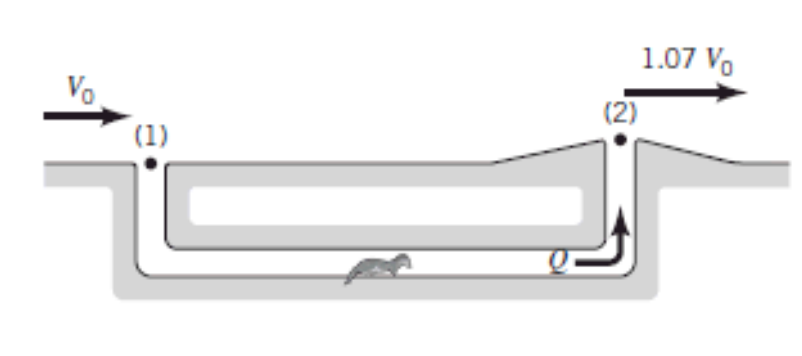
\includegraphics[width=0.5\textwidth]{3-5-2.png}
\end{center}

\textbf{Solution}
\begin{itemize}
    \item The Bernoulli equation is:
    \[p_1+\frac{1}{2}\rho V_1^2+\gamma z_1=p_2+\frac{1}{2}\rho V_2^2+\gamma z_2\]
    \item Since there are negligible gravitational effects, $z_1\approx z_2$, the Bernoulli equation is reduced to:
    \[p_1-p_2=\frac{1}{2}\rho(V_2^2-V_1^2)\]
    \[=\frac{1}{2}\left(1.23\ \frac{\mathrm{kg}}{\mathrm{m}^3}\right)\left\{\left[1.07\left(5.20\ \frac{\mathrm{m}}{\mathrm{s}}\right)\right]^2-\left[5.20\ \frac{\mathrm{m}}{\mathrm{s}}\right]^2\right\}\]
    \[\boxed{p_1-p_2=2.41\ \frac{\mathrm{N}}{\mathrm{m}^2}}\]
\end{itemize}

\textbf{Problem 3.5.3}\\
\textbf{(a)} 2013 Indianapolis 500 champion Tony Kanaan holds his hand out of his IndyCar while driving through still air with standard atmospheric conditions. For safety, the pit lane speed limit is 62 mph. At this speed, what is the maximum pressure on his hand?

\textbf{Solution}
\begin{itemize}
    \item Apply the equation:
    \[\frac{p_1}{\gamma}+\frac{V_1^2}{2g}+z_1=\frac{p_2}{\gamma}+\frac{V_2^2}{2g}+z_2\]
    \item With $z_1=z_2$, $p_1=0$, and $V_2=0$ to obtain
    \[p_2=\frac{\gamma}{2g}V_1^2\]
    \[=\frac{1}{2}\rho V_1^2\]
    \item Since
    \[V_1=(62\ \mathrm{mph})\left(1.47\ \frac{\mathrm{ft/s}}{\mathrm{mph}}\right)\]
    \[=91.14\ \frac{\mathrm{ft}}{\mathrm{s}}\]
    then
    \[p_2=\frac{1}{2}\left(2.377\times10^{-3}\ \frac{\mathrm{slug}}{\mathrm{ft}^3}\right)\left(91.14\ \frac{\mathrm{ft}}{\mathrm{s}}\right)^2\]
    \[\boxed{p_2=9.87\ \frac{\mathrm{lb}}{\mathrm{ft}^2}}\]
\end{itemize}

\textbf{(b)} What is the maximum pressure when he is driving his IndyCar at 222 mph?

\textbf{Solution}
\begin{itemize}
    \item Since
    \[V_1=(222\ \mathrm{mph})\left(1.47\ \frac{\mathrm{ft/s}}{\mathrm{mph}}\right)\]
    \[=326.34\ \frac{\mathrm{ft}}{\mathrm{s}}\]
    then
    \[p_2=\frac{1}{2}\left(2.377\times10^{-3}\ \frac{\mathrm{slug}}{\mathrm{ft}^3}\right)\left(326.34\ \frac{\mathrm{ft}}{\mathrm{s}}\right)^2\]
    \[\boxed{p_2=126.57\ \frac{\mathrm{lb}}{\mathrm{ft}^2}}\]
\end{itemize}

\textbf{(c)} On the straightaways, the IndyCar reaches speeds in excess of 237 mph. For this speed, is your solution method for the previous questions reasonable?

\textbf{Solution}
\begin{itemize}
    \item Fluid flow can be modeled as incompressible if the density change is less than 3\%. For air at standard conditions with isentropic flow, the velocity should be less than approximately $335\ \frac{\mathrm{ft}}{\mathrm{s}}$. Thus, using the (incompressible) Bernoulli's equation may not be reasonable at
    \[237\ \mathrm{mph}=(237\ \mathrm{mph})\left(1.47\ \frac{\mathrm{ft/s}}{\mathrm{mph}}\right)\]
    \[=348.39\ \frac{\mathrm{ft}}{\mathrm{s}}\]
    \item Therefore, the solution method for the previous questions is not reasonable when the IndyCar reaches speeds in excess of 237 mph.
    \[\boxed{\text{No}}\]
\end{itemize}
\section*{\fbox{3.6 Examples of use of the Bernoulli equation}}

\textbf{Problem 3.6.1}\\
The tank shown in the figure below contains air at atmospheric pressure above the water surface. The diameter of the tank is $D=10\ \mathrm{ft}$, and the velocity of the water flowing from the tank is $V_2=20.0\ \frac{\mathrm{ft}}{\mathrm{s}}$. Determine the water level $h$.

\begin{center}
    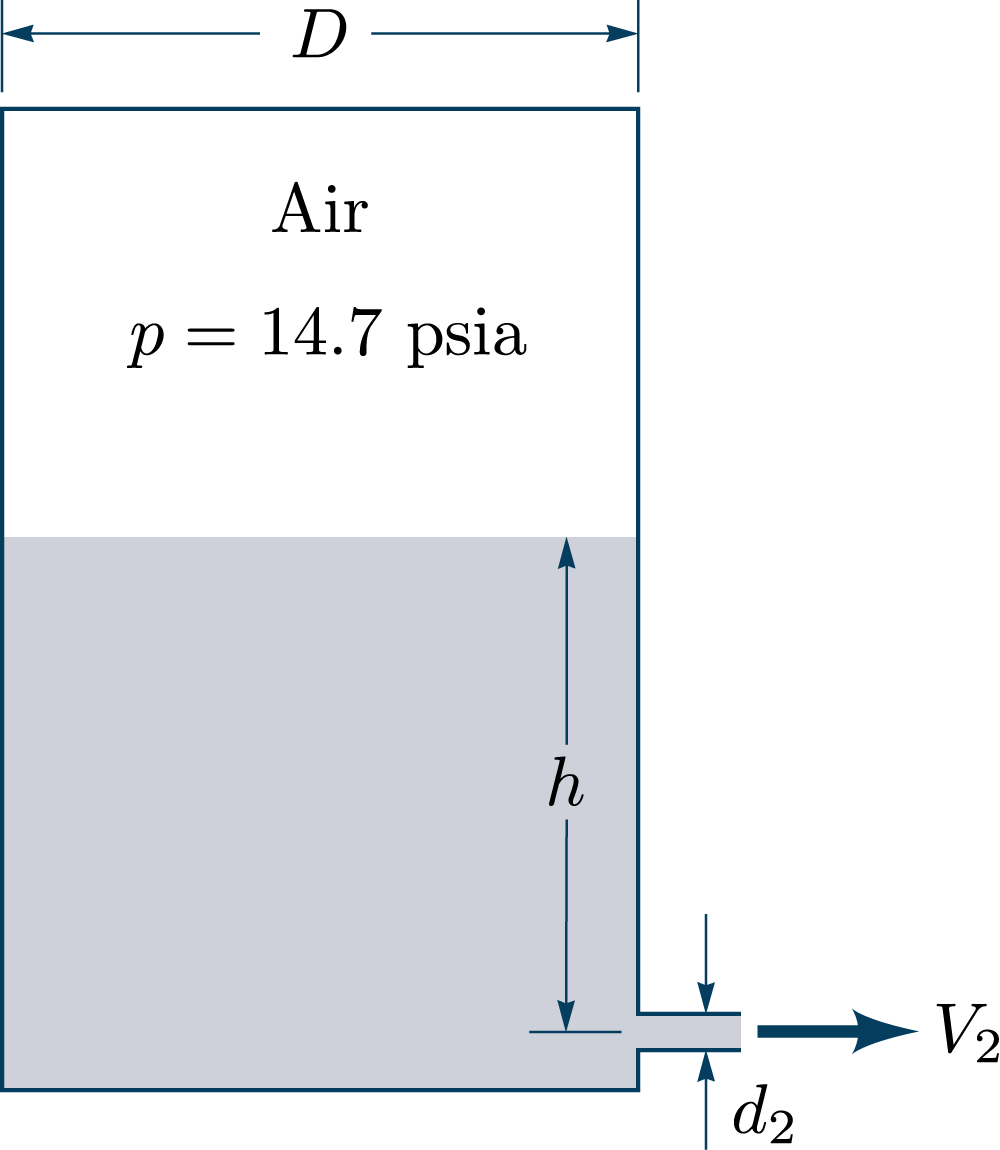
\includegraphics[width=0.3\textwidth]{3-6-1.png}
\end{center}

\textbf{Solution}
\begin{itemize}
    \item The Bernoulli equation is applied to a streamline connecting the water surface (1) to the tank outlet (2). Assume the flow is quasi-steady and the water density is constant.
    \[\frac{p_1}{\rho}+\frac{V_1^2}{2}+gz_1=\frac{p_2}{\rho}+\frac{V_2^2}{2}+gz_2\]
    where $p_1=p_2=p_{\mathrm{atm}}$ and $V_1\approx0$.
    \item Thus,
    \[g(z_1-z_2)=\frac{V_2^2}{2}\]
    and the water level $h=z_1-z_2$, so
    \[h=\frac{V_2^2}{2g}\]
    \[=\frac{\left(20.0\ \frac{\mathrm{ft}}{\mathrm{s}}\right)^2}{2\left(32.2\ \frac{\mathrm{ft}}{\mathrm{s}^2}\right)}\]
    \[\boxed{h=6.21\ \mathrm{ft}}\]
\end{itemize}


\textbf{Problem 3.6.2}\\
Water flows from the faucet on the first floor of the building shown in the figure below with a maximum velocity of $19.8\ \frac{\mathrm{ft}}{\mathrm{s}}$.

\begin{center}
    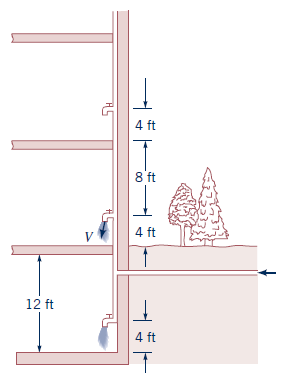
\includegraphics[width=0.4\textwidth]{3-6-2.png}
\end{center}

\textbf{(a)} For steady inviscid flow, determine the maximum water velocity from the basement faucet (assume each floor is 12 ft tall). Enter "0" in case of "no flow".

\textbf{Solution}
\begin{itemize}
    \item Since the flow is steady and inviscid, we can apply the Bernoulli equation. Since the fluid stays the same, the density is constant.
    \[\frac{p}{\gamma}+\frac{V^2}{2g}+z=\text{constant}\]
    \item Thus, the Bernoulli equation is
    \[\frac{p_1}{\gamma}+\frac{V_1^2}{2g}+z_1=\frac{p_2}{\gamma}+\frac{V_2^2}{2g}+z_2\]
    with $p_2=p_1=0$ (free jet) and $V_1=19.8\ \frac{\mathrm{ft}}{\mathrm{s}}$, $z_1=4\ \mathrm{ft}$, $z_2=-8\ \mathrm{ft}$
    \[\frac{\left(19.8\ \frac{\mathrm{ft}}{\mathrm{s}}\right)^2}{2\left(32.2\ \frac{\mathrm{ft}}{\mathrm{s}^2}\right)}+4\ \mathrm{ft}=\frac{V_2^2}{2\left(32.2\ \frac{\mathrm{ft}}{\mathrm{s}^2}\right)}+(-8\ \mathrm{ft})\]
    or
    \[\boxed{V_2=34.1\ \frac{\mathrm{ft}}{\mathrm{s}}}\]
\end{itemize}
\newpage
\textbf{(b)} For steady inviscid flow, determine the maximum water velocity from the faucet on the second floor (assume each floor is 12 ft tall). Enter "0" in case of "no flow".

\textbf{Solution}
\begin{itemize}
    \item To determine the maximum water velocity from the faucet on the second floor, use:
    \[\frac{p_1}{\gamma}+\frac{V_1^2}{2g}+z_1=\frac{p_3}{\gamma}+\frac{V_3^2}{2g}+z_3\]
    with $p_3=p_1=0$ (free jet) and $V_1=19.8\ \frac{\mathrm{ft}}{\mathrm{s}}$, $z_1=4\ \mathrm{ft}$, $z_3=16\ \mathrm{ft}$
    \[\frac{\left(19.8\ \frac{\mathrm{ft}}{\mathrm{s}}\right)^2}{2\left(32.2\ \frac{\mathrm{ft}}{\mathrm{s}^2}\right)}+4\ \mathrm{ft}=\frac{V_3^2}{2\left(32.2\ \frac{\mathrm{ft}}{\mathrm{s}^2}\right)}+(16\ \mathrm{ft})\]
    or
    \[V_3=\sqrt{19.8^2-2(32.2)(12)}\]
    \[=\sqrt{-381}\]
    \item Impossible! No flow from second floor faucet.
    \[\boxed{V_3=0\ \frac{\mathrm{ft}}{\mathrm{s}}}\]
\end{itemize}


\textbf{Problem 3.6.3}\\
An inviscid, incompressible liquid flows steadily from the large pressurized tank shown in the figure below. The velocity at the exit is $40\ \frac{\mathrm{ft}}{\mathrm{s}}$. First choose an equation to model the flow. Then, determine whether the following assumptions and conditions for the use of the Bernoulli equation are satisfied.

\begin{center}
    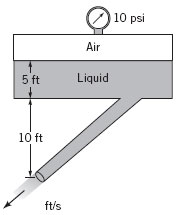
\includegraphics[width=0.25\textwidth]{3-6-3.jpeg}
\end{center}

\begin{itemize}
    \item[(a)] Can one or more streamlines be identified?
    \item[(b)] Is the flow without significant viscous effects?
    \item[(c)] Is the flow quasi-steady?
    \item[(d)] Is the flow incompressible?
    \item[(e)] Is any mechanical work done on the fluid?
\end{itemize}

\textbf{Solution}
\begin{itemize}
    \item[(a)] Yes. There is a streamline at the exit of the tank since the flow has a specified velocity $V$.
    \item[(b)] Yes. Since the flow is steady and inviscid, one can assume there are no significant viscous effects.
    \item[(c)] Yes. There is only one exit point so we can assume that the flow is steadily flowing out.
    \item[(d)] Yes. The flow is specified as incompressible in the problem statement.
    \item[(e)] No. Since the flow is considered steady, inviscid, incompressible, and there is no work being done on the fluid, we can use the Bernoulli equation to solve this problem.
\end{itemize}

\textbf{(b)} Calculate the specific weight of the unknown fluid in $\mathrm{lb/ft^3}$. The velocity at the exit is $35\ \frac{\mathrm{ft}}{\mathrm{s}}$.

\textbf{Solution}
\begin{itemize}
    \item Using the Bernoulli equation
    \[\frac{p_1}{\gamma}+z_1+\frac{V_1^2}{2g}=\frac{p_2}{\gamma}+z_2+\frac{V_2^2}{2g}\]
    where
    \[p_1=10\ \frac{\mathrm{lb}}{\mathrm{in}^2}\left(144\ \frac{\mathrm{in}^2}{\mathrm{ft}^2}\right)\]
    \[=1440\ \frac{\mathrm{lb}}{\mathrm{ft}^2}\]
    and
    \[p_2=0,\ z_1=15\ \mathrm{ft},\ z_2=0,\ V_1=0,\ V_2=35\ \frac{\mathrm{ft}}{\mathrm{s}}\]
    \item Thus,
    \[\frac{1440\ \frac{\mathrm{lb}}{\mathrm{ft}^2}}{\gamma}+15\ \mathrm{ft}=\frac{\left(35\ \frac{\mathrm{ft}}{\mathrm{s}}\right)^2}{2\left(32.2\ \frac{\mathrm{ft}}{\mathrm{s}^2}\right)}\]
    or
    \[\boxed{\gamma=358\ \frac{\mathrm{lb}}{\mathrm{ft}^3}}\]
\end{itemize}

\textbf{Problem 3.6.4}\\
Streams of water from two tanks impinge upon each other as shown in the figure below. Viscous effects are negligible and point $A$ is a stagnation point. First choose an equation to model the flow. Are the following assumptions and conditions for the use of Bernoulli's Equation satisfied?

\begin{center}
    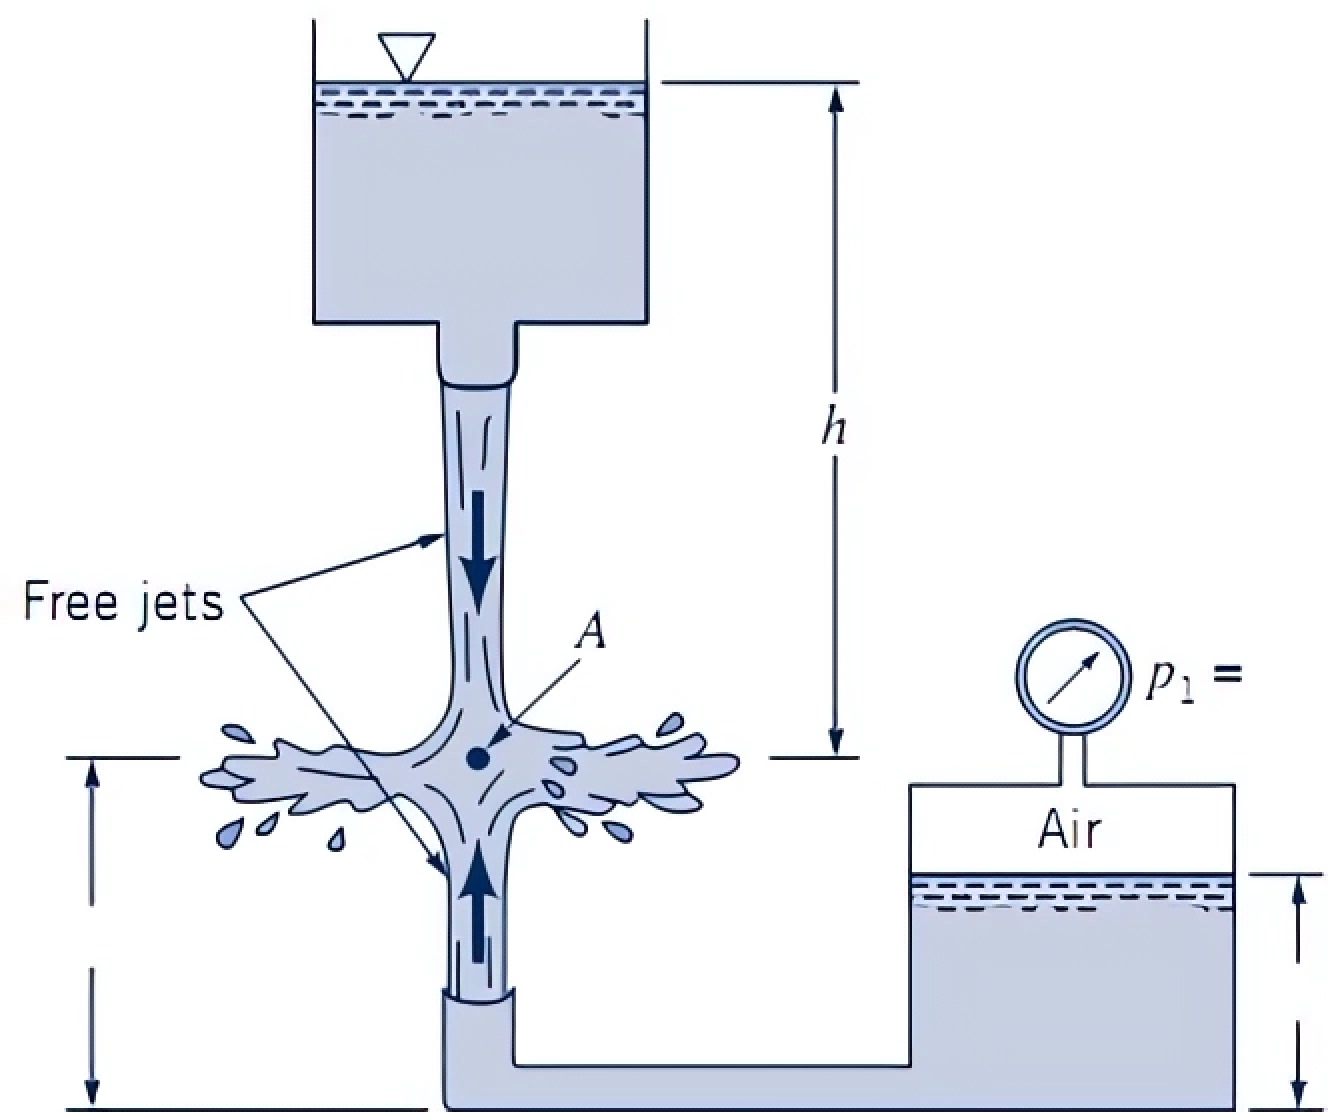
\includegraphics[width=0.5\textwidth]{3-6-4.png}
\end{center}

\begin{itemize}
    \item[(a)] Can one or more streamlines be identified?
    \item[(b)] Is the flow without significant viscous effects?
    \item[(c)] Is the flow incompressible?
    \item[(d)] Is the flow steady?
    \item[(e)] Is there any mechanical work done on the fluid?
    \item[(f)] Calculate the height, $h$.
\end{itemize}

\textbf{Solution}
\begin{itemize}
    \item[(a)] There are two specified free jets in the image, so there are streamlines.
    \item[(b)] The problem statement specifies that the viscous effects are negligible.
    \item[(c)] Two streams of water are seen and are generally assumed to be incompressible.
    \item[(d)] How the flows are arranged implies that the flow is steady.
    \item[(e)] There is no change in mechanical energy, so no mechanical work is being done on the fluid.
    \item[(f)] Using the Bernoulli equation, we can begin to solve this problem.
    \[\frac{p_2}{\gamma}+\frac{V_2^2}{2g}+z_2=\frac{p_A}{\gamma}+\frac{V_A^2}{2g}+z_A\]
    where $p_2=0$, $V_2=0$, $z_2=h+15\ \mathrm{ft}$, $V_A=0$, and $z_A=15\ \mathrm{ft}$. Thus,
    \[h+15\ \mathrm{ft}=\frac{p_A}{\gamma}+15\ \mathrm{ft}\]
    \[h=\frac{p_A}{\gamma}\tag{Eq. 1}\]
    Also,
    \[\frac{p_1}{\gamma}+\frac{V_1^2}{2g}+z_1=\frac{p_A}{\gamma}+\frac{V_A^2}{2g}+z_A\]
    where $p_1=23\ \mathrm{psi}$, $V_1=0$, and $z_1=8\ \mathrm{ft}$.

    Thus,
    \[\frac{p_A}{\gamma}=\frac{p_1}{\gamma}+z_1-z_A\]
    which when combined with Eq. 1, gives
    \[h=\frac{p_1}{\gamma}+z_1-z_A\]
    \[=\frac{23\ \frac{\mathrm{lb}}{\mathrm{in}^2}\left(144\ \frac{\mathrm{in}^2}{\mathrm{ft}^2}\right)}{62.4\ \frac{\mathrm{lb}}{\mathrm{ft}^3}}+8\ \mathrm{ft}-15\ \mathrm{ft}\]
    \[\boxed{h=46.1\ \mathrm{ft}}\]
\end{itemize}

\textbf{Problem 3.6.5}\\
A fire hose nozzle has an outlet diameter of 1.1 in and is attached to a 3.6-in.-diameter hose. According to some fire codes, the nozzle must be capable of delivering at least $250\ \frac{\mathrm{gal}}{\mathrm{min}}$.

\begin{center}
    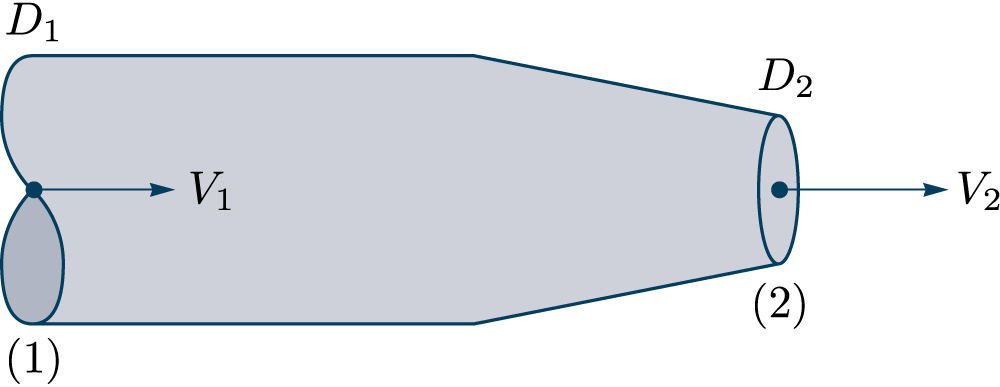
\includegraphics[width=0.4\textwidth]{3-6-5.png}
\end{center}

\textbf{(a)} Determine the velocity at the nozzle inlet when $Q=250\ \frac{\mathrm{gal}}{\mathrm{min}}$.

\textbf{(b)} Determine the velocity at the nozzle outlet when $Q=250\ \frac{\mathrm{gal}}{\mathrm{min}}$.

\textbf{Solution}
\begin{itemize}
    \item The flowrate $Q$ is converted from $\frac{\mathrm{gal}}{\mathrm{min}}$ to $\frac{\mathrm{ft}^3}{\mathrm{s}}$.
    \[Q=\left(250\ \frac{\mathrm{gal}}{\mathrm{min}}\right)\left(\frac{231\ \mathrm{in.}^3}{1\ \mathrm{gal}}\right)\left(\frac{1\ \mathrm{ft}^3}{1728\ \mathrm{in.}^3}\right)\left(\frac{1\ \mathrm{min}}{60\ \mathrm{s}}\right)\]
    \[=0.557\ \frac{\mathrm{ft}^3}{\mathrm{s}}\]
    \item Then, $Q$ is used to calculate the velocity since $Q=VA$.
    \item[(a)] The velocity at the nozzle inlet is
    \[V_1=\frac{Q}{A_1}\]
    \[=\frac{0.557\ \frac{\mathrm{ft}^3}{\mathrm{s}}}{\frac{\pi}{4}(3.6\ \mathrm{in.})^2\left(\frac{1\ \mathrm{ft}^2}{144\ \mathrm{in.}^2}\right)}\]
    \[\boxed{V_1=7.88\ \frac{\mathrm{ft}}{\mathrm{s}}}\]
    \item[(b)] The velocity at the nozzle outlet is
    \[V_2=\frac{Q}{A_2}\]
    \[=\frac{0.557\ \frac{\mathrm{ft}^3}{\mathrm{s}}}{\frac{\pi}{4}(1.1\ \mathrm{in.})^2\left(\frac{1\ \mathrm{ft}^2}{144\ \mathrm{in.}^2}\right)}\]
    \[\boxed{V_2=84.4\ \frac{\mathrm{ft}}{\mathrm{s}}}\]
\end{itemize}

\textbf{(c)} A fire hose nozzle has an outlet diameter of 1.6 in. If the nozzle is attached to a 3.1-in.-diameter hose, determine the pressure that must be maintained just upstream of the nozzle to deliver the flowrate $Q=250\ \frac{\mathrm{gal}}{\mathrm{min}}$.

\textbf{Solution}
\begin{itemize}
    \item The Bernoulli equation is applied between the inlet and the outlet of the fire hose nozzle.
    \[\frac{p_1}{\gamma}+\frac{V_1^2}{2g}+z_1=\frac{p_2}{\gamma}+\frac{V_2^2}{2g}+z_2\]
    where $z_1=z_2$ and $p_2=0\ \mathrm{psig}$.
    \item Rearranging the Bernoulli equation gives:
    \[p_1=\frac{\gamma}{2g}[V_2^2-V_1^2]\]
    where
    \[V_2=\frac{Q}{A_2}=\frac{0.557\ \frac{\mathrm{ft}^3}{\mathrm{s}}}{\frac{\pi}{4}(1.6\ \mathrm{in.})^2\left(\frac{1\ \mathrm{ft}^2}{144\ \mathrm{in.}^2}\right)}\]
    \[=39.9\ \frac{\mathrm{ft}}{\mathrm{s}}\]
    and
    \[V_1=\frac{Q}{A_1}=\frac{0.557\ \frac{\mathrm{ft}^3}{\mathrm{s}}}{\frac{\pi}{4}(3.1\ \mathrm{in.})^2\left(\frac{1\ \mathrm{ft}^2}{144\ \mathrm{in.}^2}\right)}\]
    \[=10.6\ \frac{\mathrm{ft}}{\mathrm{s}}\]
    \item Thus, with $\frac{\gamma}{g}=\rho$, the inlet pressure is
    \[p_1=\frac{1}{2}\left(1.94\ \frac{\mathrm{slugs}}{\mathrm{ft}^3}\right)[39.9^2-10.6^2]\ \frac{\mathrm{ft}^2}{\mathrm{s}^2}\]
    \[=1430\ \frac{\mathrm{lb}}{\mathrm{ft}^2}\left(\frac{1\ \mathrm{ft}^2}{144\ \mathrm{in.}^2}\right)\]
    \[\boxed{p_1=9.96\ \mathrm{psig}}\]
\end{itemize}

\textbf{Problem 3.6.6}\\
Water (assumed inviscid and incompressible) flows steadily with a speed of $6\ \frac{\mathrm{ft}}{\mathrm{s}}$ from the large tank shown in the figure below. Determine the depth, $H$, of the layer of light liquid that covers the water in the tank.

\begin{center}
    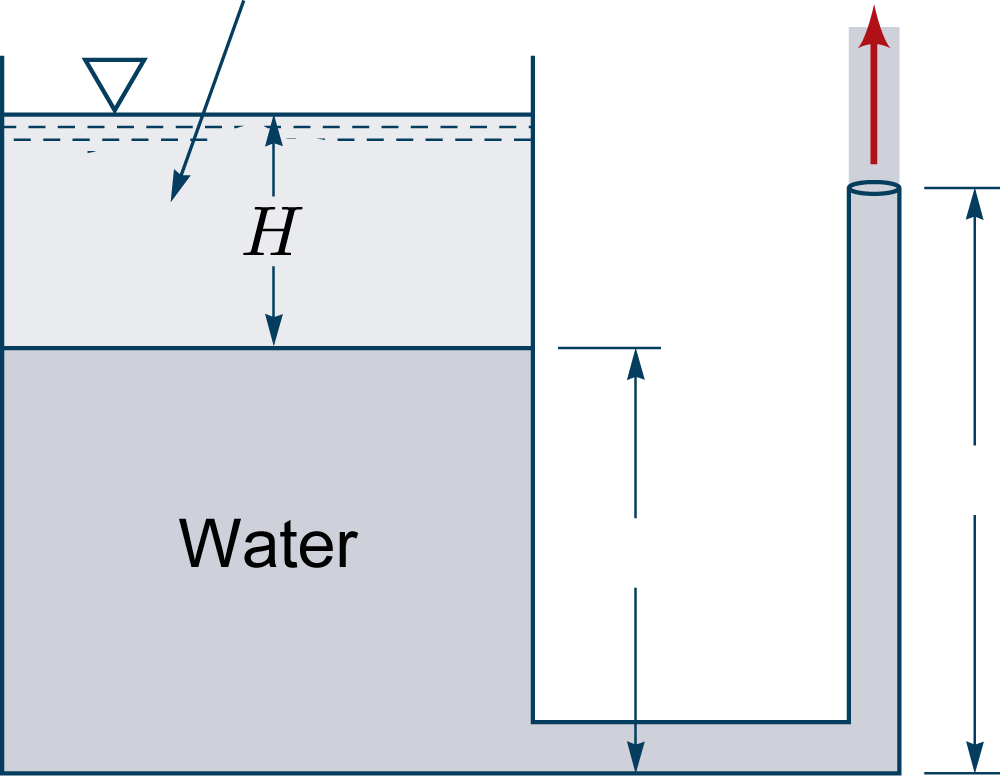
\includegraphics[width=0.4\textwidth]{3-6-6.png}
\end{center}

\textbf{Solution}
\begin{itemize}
    \item The Bernoulli equation is applied between the water surface in the container and the top of the jet exiting the pipe.
    \[\frac{p_1}{\gamma}+\frac{V_1^2}{2g}+z_1=\frac{p_2}{\gamma}+\frac{V_2^2}{2g}+z_2\]
    where $p_1=\gamma_oH$, $V_1=0$, $p_2=0$, $z_1=3\ \mathrm{ft}$, and $z_2=4\ \mathrm{ft}$. Thus,
    \[\frac{\gamma_oH}{\gamma}+z_1=\frac{V_2^2}{2g}+z_2\]
    \item With $V_2=6\ \frac{\mathrm{ft}}{\mathrm{s}}$,
    \[\left[\frac{46\ \frac{\mathrm{lb}}{\mathrm{ft}^3}}{62.4\ \frac{\mathrm{lb}}{\mathrm{ft}^3}}\right]H+3\ \mathrm{ft}=\frac{\left(6\ \frac{\mathrm{ft}}{\mathrm{s}}\right)^2}{2\left(32.2\ \frac{\mathrm{ft}}{\mathrm{s}^2}\right)}+4\ \mathrm{ft}\]
    \item Therefore,
    \[\boxed{H=2.11\ \mathrm{ft}}\]
\end{itemize}


\textbf{Problem 3.6.7}\\
Water flows through the pipe contraction shown in the figure below. The inlet diameter is $D_1=0.3\ \mathrm{m}$. Determine the flowrate if the difference in the manometer levels is $h=0.36\ \mathrm{m}$.

\begin{center}
    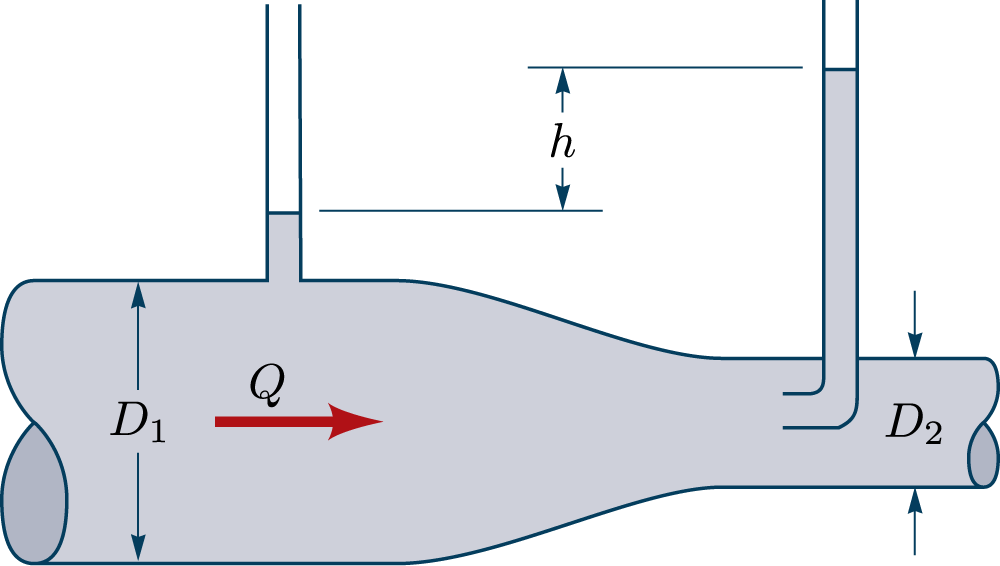
\includegraphics[width=0.4\textwidth]{3-6-7.png}
\end{center}

\textbf{Solution}
\begin{itemize}
    \item The Bernoulli equation is applied between points (1) and (2) in the figure below.
    \begin{center}
        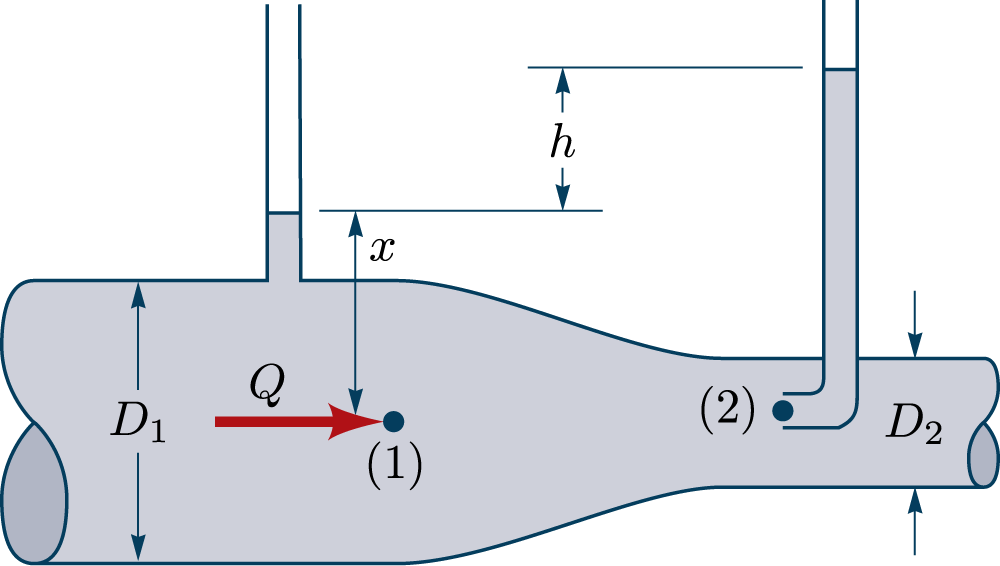
\includegraphics[width=0.4\textwidth]{3-6-7_1.png}
    \end{center}
    \[\frac{p_1}{\gamma}+\frac{V_1^2}{2g}+z_1=\frac{p_2}{\gamma}+\frac{V_2^2}{2g}+z_2\]
    or,
    \[\frac{V_1^2}{2g}=\frac{p_2}{\gamma}+\frac{V_2^2}{2g}-\frac{p_1}{\gamma}\]
    with $\frac{p_1}{\gamma}=x$ and $\frac{p_2}{\gamma}+ \frac{V_2^2}{2g}=h+x$, the equation becomes
    \[\frac{V_1^2}{2g}=h+x-x\]
    or
    \[V_1=\sqrt{2gh}\]
    \[=\sqrt{2\left(9.81\ \frac{\mathrm{m}}{\mathrm{s}^2}\right)(0.36\ \mathrm{m})}\]
    \[=2.66\ \frac{\mathrm{m}}{\mathrm{s}}\]
    \item Finally,
    \[Q=A_1V_1\]
    \[=\frac{\pi}{4}(0.3\ \mathrm{m})^2\left(2.66\ \frac{\mathrm{m}}{\mathrm{s}}\right)\]
    \[\boxed{Q=0.188\ \frac{\mathrm{m}^3}{\mathrm{s}}}\]
\end{itemize}


\textbf{Problem 3.6.8}\\
Water flows under the inclined sluice gate shown in the figure below. Determine the flowrate if the sluice gate is 9 ft wide.

\begin{center}
    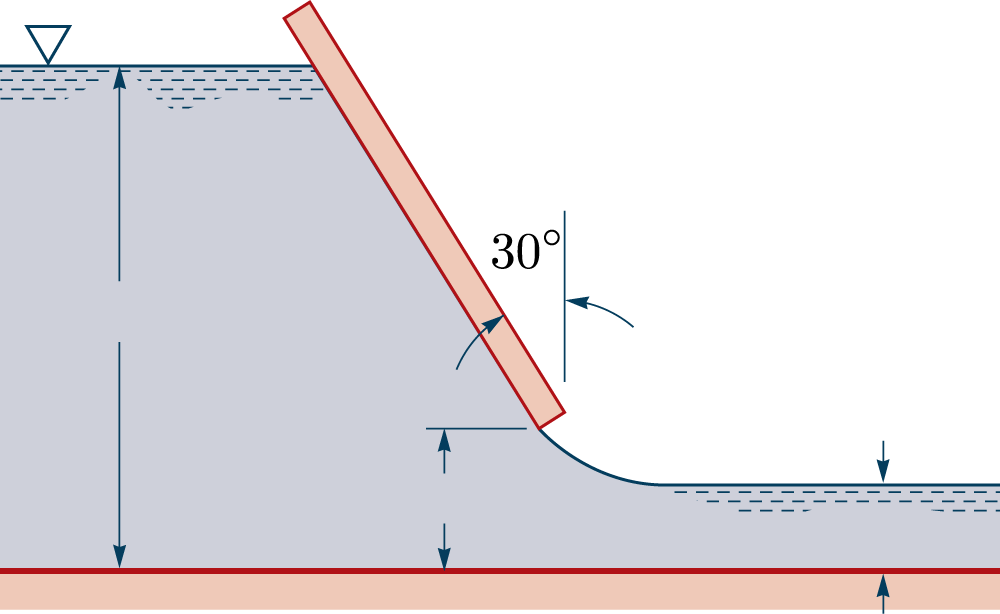
\includegraphics[width=0.4\textwidth]{3-6-8.png}
\end{center}

\textbf{Solution}
\begin{itemize}
    \item
    \[Q=z_3b\sqrt{\frac{2g(z_1-z_3)}{1-\left(\frac{z_3}{z_1}\right)^2}}\]
    where $z_1=6.1\ \mathrm{ft}$, $z_3=1.1\ \mathrm{ft}$, and $b=9\ \mathrm{ft}$.
    \item Thus,
    \[Q=(1.1\ \mathrm{ft})(9\ \mathrm{ft})\sqrt{\frac{2\left(32.2\ \frac{\mathrm{ft}}{\mathrm{s}^2}\right)(6.1\ \mathrm{ft}-1.1\ \mathrm{ft})}{1-\left(\frac{1.1\ \mathrm{ft}}{6.1\ \mathrm{ft}}\right)^2}}\]
    \[\boxed{Q=181\ \frac{\mathrm{ft}^3}{\mathrm{s}}}\]
\end{itemize}
\newpage
\section*{\fbox{3.7 The energy line and the hydraulic grade line}}

\textbf{Problem 3.7.1}\\
Water flows in a 0.16-m-diameter vertical pipe at a rate of $0.40\ \frac{\mathrm{m}^3}{\mathrm{s}}$ and a pressure of 230 kPa at an elevation of $z_1=21\ \mathrm{m}$.

\begin{center}
    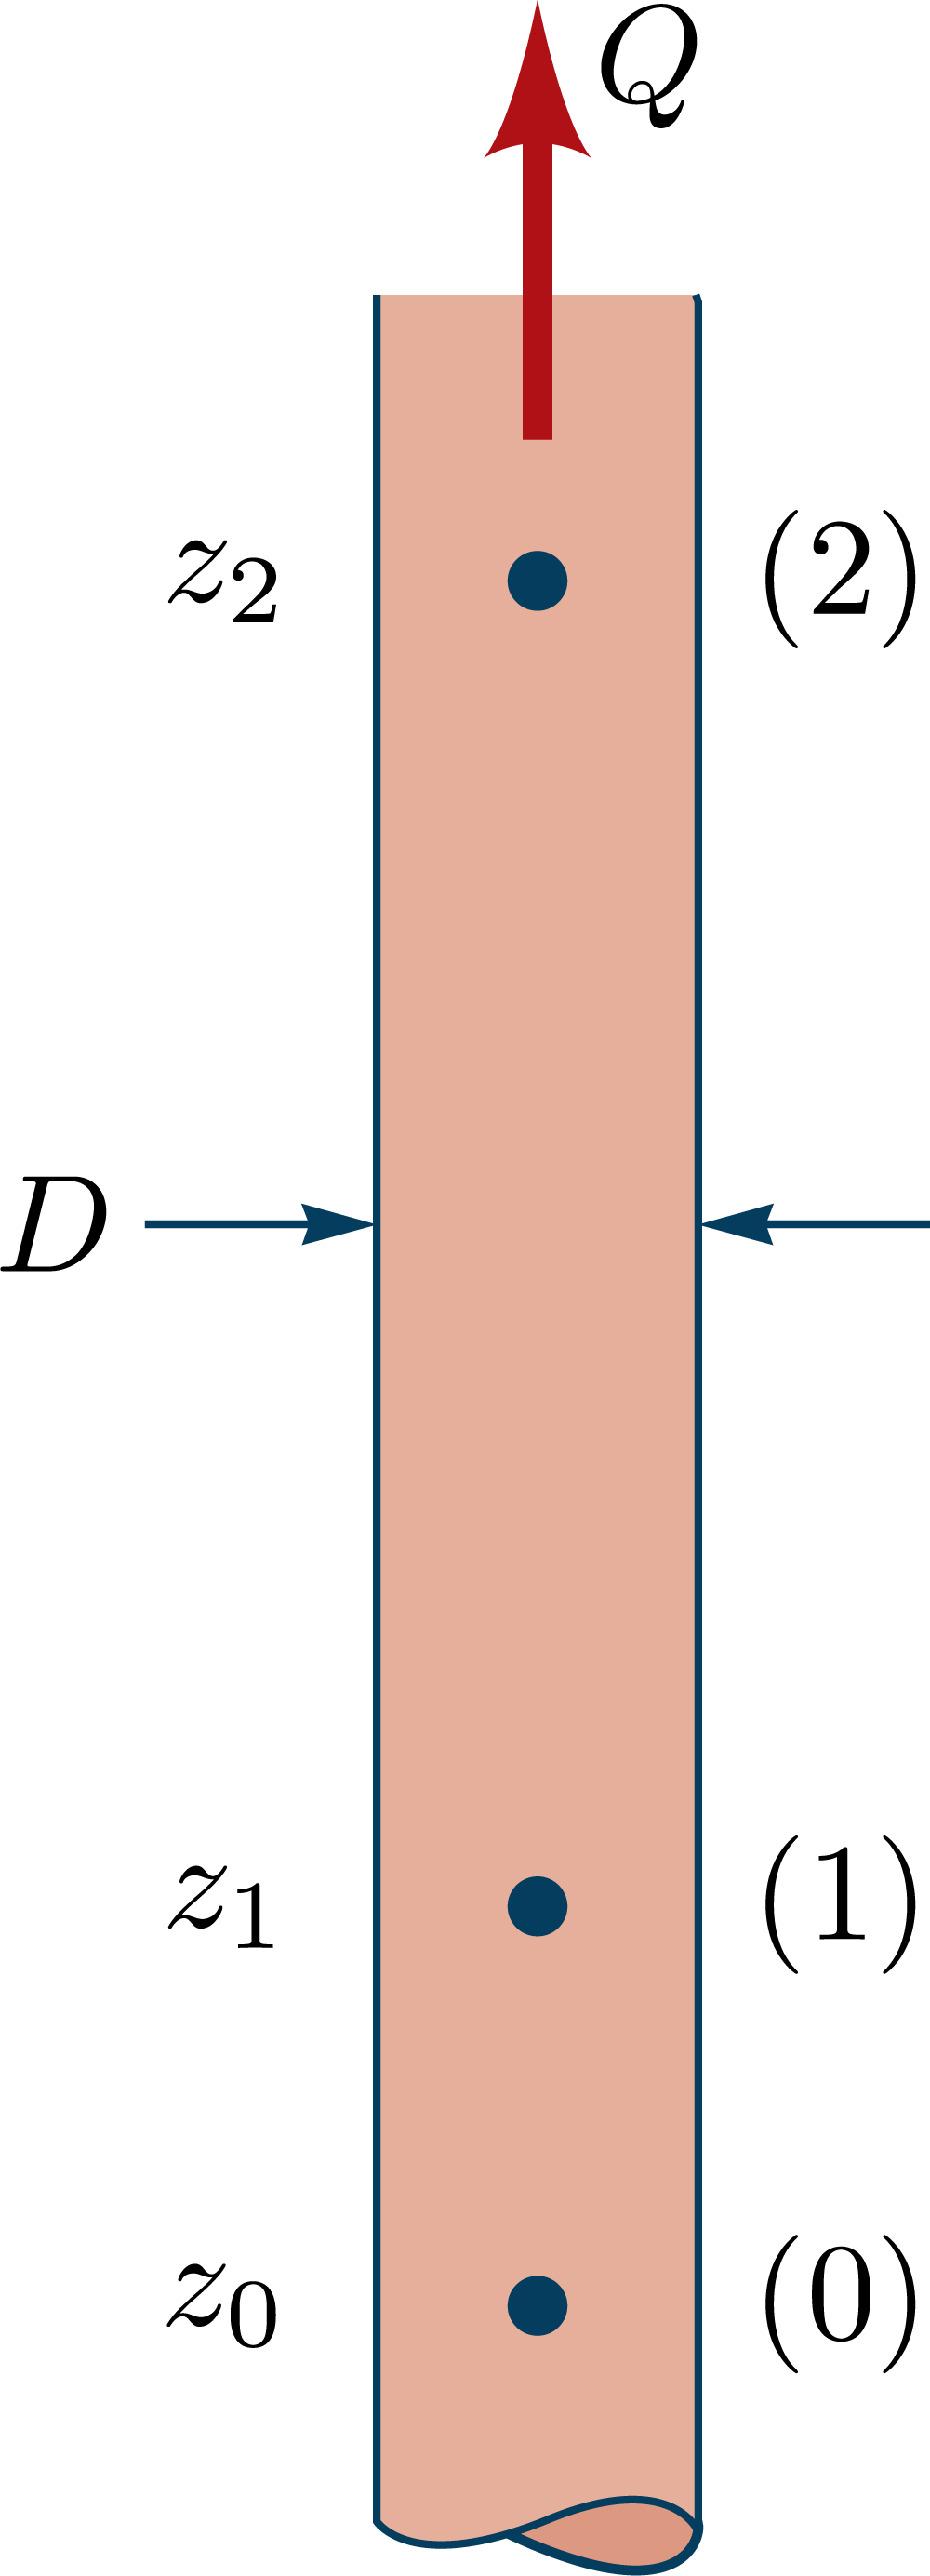
\includegraphics[width=0.15\textwidth]{3-7-1.png}
\end{center}

\textbf{(a)} Determine the velocity head at an elevation of $z_0=15\ \mathrm{m}$.

\textbf{(b)} Determine the velocity head at an elevation of $z_2=57\ \mathrm{m}$.

\textbf{Solution}
\begin{itemize}
    \item The velocity through the pipe is found from the flow rate.
    \[V=\frac{Q}{A}\]
    \[=\frac{0.40\ \frac{\mathrm{m}^3}{\mathrm{s}}}{\pi\left(\frac{0.16\ \mathrm{m}}{2}\right)^2}\]
    \[=19.9\ \frac{\mathrm{m}}{\mathrm{s}}\]
    \item Since the flowrate is constant and the pipe diameter does not change, the velocity is constant throughout the pipe. So, $V=V_0=V_2$.
    \item The velocity head is:
    \[\frac{V^2}{2g}\]
    \item[(a)] For the elevation of $z_0=15\ \mathrm{m}$, the velocity head is:
    \[\frac{V_0^2}{2g}=\frac{\left(19.9\ \frac{\mathrm{m}}{\mathrm{s}}\right)^2}{2\left(9.81\ \frac{\mathrm{m}}{\mathrm{s}^2}\right)}\]
    \[\boxed{=20.2\ \mathrm{m}}\]
    \item[(b)] For the elevation of $z_2=57\ \mathrm{m}$, the velocity head is:
    \[\frac{V_2^2}{2g}=\frac{\left(19.9\ \frac{\mathrm{m}}{\mathrm{s}}\right)^2}{2\left(9.81\ \frac{\mathrm{m}}{\mathrm{s}^2}\right)}\]
    \[\boxed{=20.2\ \mathrm{m}}\]
\end{itemize}

\textbf{(c)} Water flows in a 0.13-m-diameter vertical pipe at a rate of $0.25\ \frac{\mathrm{m}^3}{\mathrm{s}}$ and a pressure of 260 kPa at an elevation of $z_1=21\ \mathrm{m}$. Determine the pressure head at an elevation of $z_0=13\ \mathrm{m}$.

\textbf{(d)} Determine the pressure head at an elevation of $z_2=53\ \mathrm{m}$.

\textbf{Solution}
\begin{itemize}
    \item Since the flowrate is constant and the pipe diameter does not change, the velocity is constant throughout the pipe.
    \item[(c)] The pressure head at an elevation of $z_0=13\ \mathrm{m}$ is found using the Bernoulli equation between points (0) and (1).
    \[\frac{p_0}{\gamma}+\frac{V_0^2}{2g}+z_0=\frac{p_1}{\gamma}+\frac{V_1^2}{2g}+z_1\]
    \item Since $V=V_0=V_1$, the pressure head is:
    \[\frac{p_0}{\gamma}=\frac{p_1}{\gamma}+z_1-z_0\]
    \[=\frac{260\ \frac{\mathrm{kN}}{\mathrm{m}^2}}{9.8\ \frac{\mathrm{kN}}{\mathrm{m}^3}}+21\ \mathrm{m}-13\ \mathrm{m}\]
    \[\boxed{=34.5\ \mathrm{m}}\]
    \item[(d)] Similarly, the pressure head at an elevation of $z_2=53\ \mathrm{m}$ is found using the Bernoulli equation between points (1) and (2).
    \[\frac{p_2}{\gamma}+\frac{V_2^2}{2g}+z_2=\frac{p_1}{\gamma}+\frac{V_1^2}{2g}+z_1\]
    \item Since $V=V_1=V_2$, the pressure head is:
    \[\frac{p_2}{\gamma}=\frac{p_1}{\gamma}+z_1-z_2\]
    \[=\frac{260\ \frac{\mathrm{kN}}{\mathrm{m}^2}}{9.8\ \frac{\mathrm{kN}}{\mathrm{m}^3}}+21\ \mathrm{m}-53\ \mathrm{m}\]
    \[\boxed{=-5.47\ \mathrm{m}}\]
\end{itemize}


\textbf{Problem 3.7.2}\\
A smooth plastic, 10 m long garden hose with an inside diameter of 20 mm is used to drain a wading pool as shown in the figure. $h_1=0.36\ \mathrm{m}$ and $h_2=0.62\ \mathrm{m}$. Choose the number of the energy line and hydraulic grade line for the flow shown below.
\begin{center}
    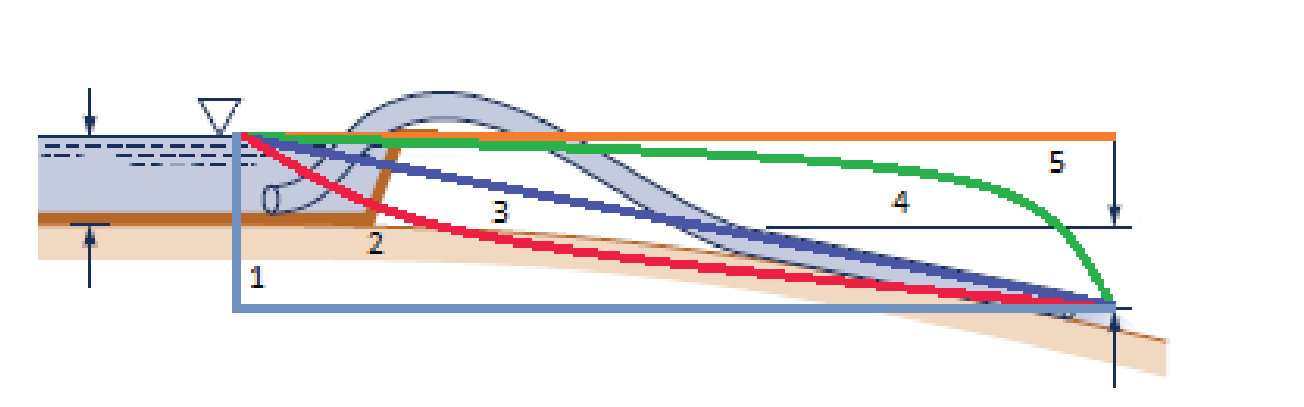
\includegraphics[width=0.7\textwidth]{3-7-2_1.png}
\end{center}

\begin{itemize}
    \item[(a)] Find $\frac{V_2^2}{2g}$.
    \item[(b)] The energy line (EL).
    \item[(c)] The hydraulic grade line (HGL).
\end{itemize}
\textbf{Solution}
\begin{itemize}
    \item (a), (b), (c) Draw the energy line and hydraulic grade line for the flow shown above.
    \item Since
    \[\frac{p_1}{\gamma}+\frac{V_1^2}{2g}+Z_1=\frac{p_2}{\gamma}+\frac{V_2^2}{2g}+Z_2\]
    with $p_1=p_2=0$, $V_1=0$, $Z_2=0$
    \item and,
    \[Z_1=0.36\ \mathrm{m}+0.62\ \mathrm{m}=0.98\ \mathrm{m}\]
    it follows that
    \[\boxed{\frac{V_2^2}{2g}=0.98\ \mathrm{m}}\]
    \item Since the fluid velocity is constant throughout the pipe with $\frac{V_2^2}{2g}=0.98\ \mathrm{m}$, the diagram below is obtained.

    \begin{center}
        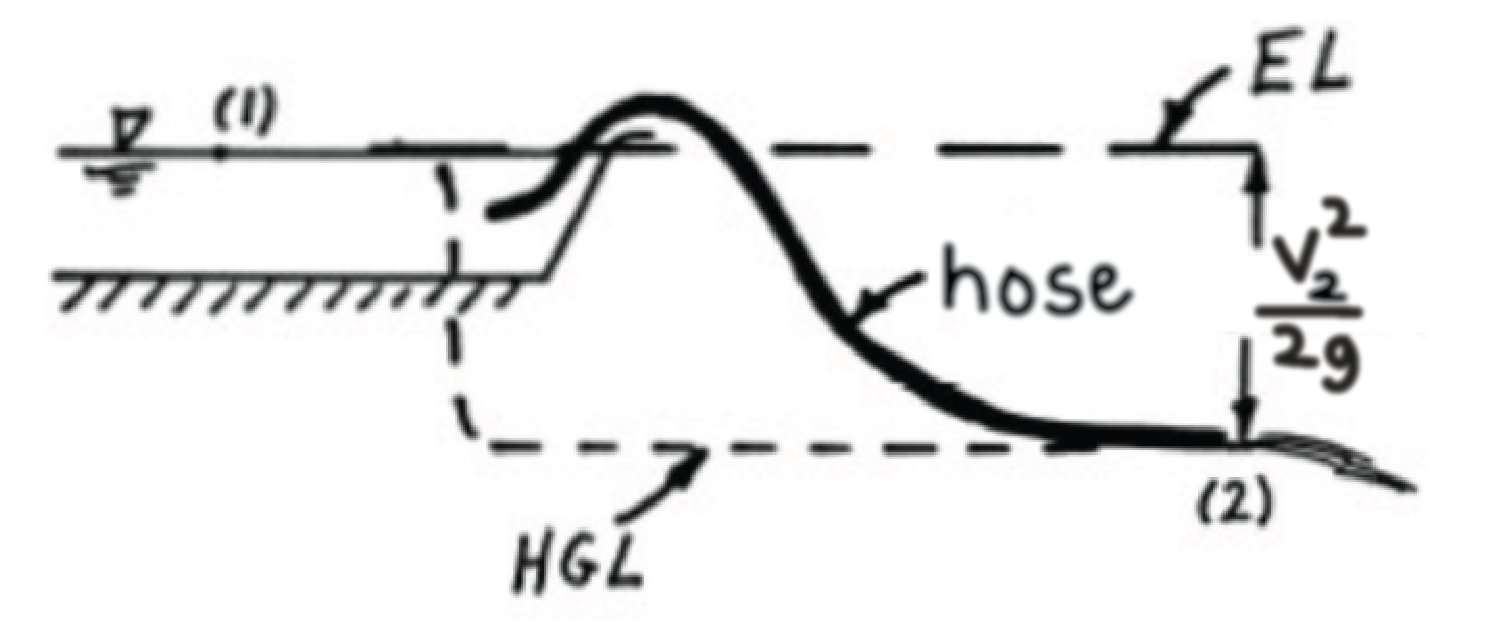
\includegraphics[width=0.5\textwidth]{3-7-2_2.png}
    \end{center}

    \item For inviscid flow with no pumps or turbines, the energy line (EL) is horizontal, at an elevation of the free surface, consistent with energy line 5. The hydraulic grade line (HGL) is one velocity head lower, even with the pipe outlet, consistent with hydraulic grade line 1.
    \[\boxed{\text{EL}=5}\]
    \[\boxed{\text{HGL}=1}\]
\end{itemize}

\textbf{Participation Activity 3.7.1}\\
The pipe shown below has three sections 1, 2 and 3. Section 1 converges to section 2 and section 2 diverges to section 3.

\begin{center}
    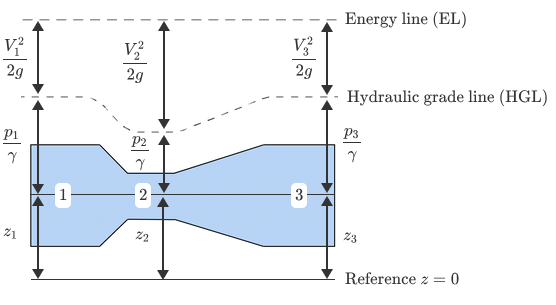
\includegraphics[width=0.6\textwidth]{3-7-1 ex.png}
\end{center}

\begin{itemize}
    \item Assuming inviscid, steady, and incompressible flow, the Bernoulli equation can be used.
    \[\frac{p}{\gamma}+\frac{V^2}{2g}+z=\text{Constant along a streamline}\]
    \item The energy line (EL) equals the summation of $\frac{p}{\gamma}+\frac{V^2}{2g}+z$ and represents the total head. Therefore for section 1,
    \[\mathrm{EL}=\frac{p_1}{\gamma}+\frac{V_1^2}{2g}+z_1\]
    \item Since EL is constant along a streamline, EL is the same for sections 1, 2, and 3. The EL line is obtained by measuring stagnation pressure with a pitot tube and adding elevation head $z$.
    \item The hydraulic grade line (HGL) equals the summation of $\frac{p}{\gamma}$ and elevation $z$. The HGL line varies along a streamline and can be measured with a piezometer tube.
    \[\mathrm{HGL}=\frac{p}{\gamma}+z\]
\end{itemize}

\section*{\fbox{3.8 Restrictions on use of the Bernoulli equation}}

\textbf{Problem 3.8.1}\\
Water is in a 4.0 m long U-tube. (a) What is the angular frequency $\omega$? (b) What is the period $T$? (c) What is the frequency of oscillation $f$?
\newpage
\textbf{Solution}
\begin{itemize}
    \item[(a)] Using the formula for angular frequency:
    \[\boxed{\omega=\sqrt{\frac{2g}{L}}=\sqrt{\frac{2(9.81\ \mathrm{m/s^2})}{4.0\ \mathrm{m}}}=2.21\ \mathrm{rad/s}}\]
    \item[(b)] Using the formula for period:
    \[\boxed{T=2\pi\sqrt{\frac{L}{2g}}=2\pi\sqrt{\frac{4.0\ \mathrm{m}}{2(9.81\ \mathrm{m/s^2})}}=2.84\ \mathrm{s}}\]
    \item[(c)] Using the formula for the frequency of oscillation:
    \[\boxed{f=\frac{1}{T}=\frac{1}{2.84\ \mathrm{s}}=0.353\ \mathrm{Hz}}\]
\end{itemize}

\textbf{Example 3.8.2}\\
A submarine moves through seawater ($SG=1.03$) at a depth of 50 m with velocity $V_0=5.0\ \mathrm{m/s}$ as shown below. Determine the pressure at the stagnation point (2).

\begin{center}
    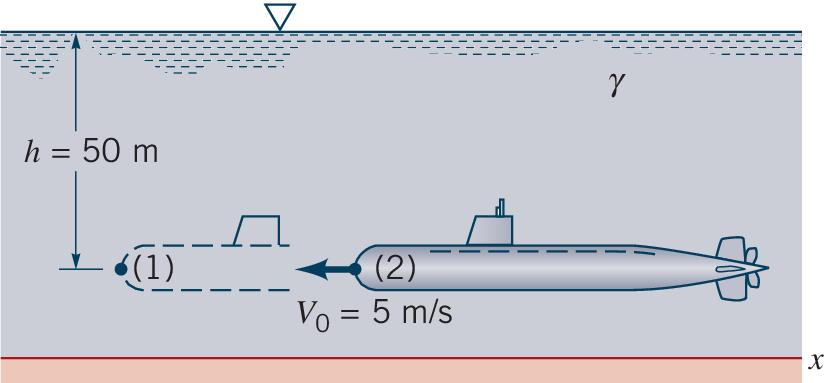
\includegraphics[width=0.5\textwidth]{3-8-2.jpeg}
\end{center}

\textbf{Solution}
\begin{itemize}
    \item In a coordinate system fixed to the ground, the flow is unsteady. For example, the water velocity at (1) is zero with the submarine in its initial position, but at the instant when the nose, (2), reaches point (1) the velocity there becomes $\mathbf{V}_1=-V_0\hat{\mathbf{i}}$. Thus, $\partial\mathbf{V}_1/\partial t\neq0$, and the flow is unsteady. Application of the steady Bernoulli equation between (1) and (2) would give the incorrect result that $p_1=p_2+\rho V_0^2/2$. According to this result, the static pressure is greater than the stagnation pressure, an incorrect use of the Bernoulli equation.
    \item We can either use an unsteady analysis for the flow (which is outside the scope of this text) or redefine the coordinate system so that it is fixed on the submarine, giving steady flow with respect to this system. The correct method would be
    \[p_2=\frac{\rho V_1^2}{2}+\gamma h=[(1.03)(1000)\ \mathrm{kg/m^3}](5.0\ \mathrm{m/s})^2/2+(9.80\times10^3\ \mathrm{N/m^3})(1.03)(50\ \mathrm{m})\]
    \[=(12,900+505,000)\ \mathrm{N/m^2}\]
    \[\boxed{p_2=518\ \mathrm{kPa}}\]
    similar to that discussed in Example 3.2.2.
    \item If the submarine were accelerating, $\partial\mathbf{V}_0/\partial t\neq0$, the flow would be unsteady in either of the coordinate systems mentioned in this example, and we would be forced to use an unsteady form of the Bernoulli equation.
\end{itemize}





\end{document}
